\documentclass[a4paper, 11pt]{article}
\usepackage[spanish]{babel}
\selectlanguage{spanish}
\usepackage{graphicx}
\usepackage{wrapfig}
\usepackage[utf8]{inputenc}
\usepackage{amsmath}
\usepackage{dsfont}
\usepackage{multirow}
\usepackage{vmargin}
\usepackage{subfigure}
\usepackage{url}
\usepackage{cite}
\usepackage{wrapfig}
\usepackage{enumerate} 
\usepackage{caption}
\usepackage{amsfonts}
\usepackage{amssymb}
\usepackage{listings}
\usepackage{color}
\usepackage{float}

\spanishdecimal{.}

\setmargins
{2.5cm}                        % margen izquierdo
{1cm}                         % margen superior
{16.5cm}                      % anchura del texto
{23.42cm}                    % altura del texto
{10pt}                           % altura de los encabezados
{0cm}                           % espacio entre el texto y los encabezados
{0pt}                             % altura del pie de página
{1cm}                           % espacio entre el texto y el pie de página

\definecolor{mygreen}{rgb}{0,0.6,0}
\definecolor{mygray}{rgb}{0.5,0.5,0.5}
\definecolor{mymauve}{rgb}{0.58,0,0.82}

\lstset{ 
  backgroundcolor=\color{white},   % choose the background color; you must add \usepackage{color} or \usepackage{xcolor}; should come as last argument
  basicstyle=\footnotesize,        % the size of the fonts that are used for the code
  breakatwhitespace=false,         % sets if automatic breaks should only happen at whitespace
  breaklines=true,                 % sets automatic line breaking
  captionpos=b,                    % sets the caption-position to bottom
  commentstyle=\color{mygreen},    % comment style
  deletekeywords={...},            % if you want to delete keywords from the given language
  escapeinside={\%*}{*)},          % if you want to add LaTeX within your code
  extendedchars=true,              % lets you use non-ASCII characters; for 8-bits encodings only, does not work with UTF-8
  firstnumber=1,                % start line enumeration with line 1000
  frame=single,	                   % adds a frame around the code
  keepspaces=true,                 % keeps spaces in text, useful for keeping indentation of code (possibly needs columns=flexible)
  keywordstyle=\color{blue},       % keyword style
  language=Octave,                 % the language of the code
  morekeywords={*,...},            % if you want to add more keywords to the set
  numbers=left,                    % where to put the line-numbers; possible values are (none, left, right)
  numbersep=5pt,                   % how far the line-numbers are from the code
  numberstyle=\tiny\color{mygray}, % the style that is used for the line-numbers
  rulecolor=\color{black},         % if not set, the frame-color may be changed on line-breaks within not-black text (e.g. comments (green here))
  showspaces=false,                % show spaces everywhere adding particular underscores; it overrides 'showstringspaces'
  showstringspaces=false,          % underline spaces within strings only
  showtabs=false,                  % show tabs within strings adding particular underscores
  stepnumber=1,                    % the step between two line-numbers. If it's 1, each line will be numbered
  stringstyle=\color{mymauve},     % string literal style
  tabsize=2,	                   % sets default tabsize to 2 spaces
  title=\lstname                   % show the filename of files included with \lstinputlisting; also try caption instead of title
}


\begin{document}

\title{Caracterización estructural de instancias}
\author{Matr\'icula: 1985281}
\date{ }
\maketitle

\vspace{-1 cm}
\begin{center}\rule{\textwidth}{0.1mm} \end{center}
\vspace{-1.3 cm}
\begin {center}
\item \Large{\textbf{ Resumen}}
\end {center}

Entre los generadores de grafos que proporciona \color{blue} NetworkX\color{black}, se seleccionó \texttt{random\_geometric\_graph} (grafo geométrico aleatorio) y la función \texttt{preflow\_push} para calcular el flujo máximo entre un par de nodos, ya que resulta ser la más eficiente para este tipo de grafos. Además, se escogieron los grafos geométricos aleatorios, ya que se suelen utilizar para representar redes de sensores inalámbricos (inglés: wireless sensor networks (WSN)).
\vspace{-0.5cm}
\begin{center}\rule{\textwidth}{0.1mm} \end{center}




\section*{\centering{Introducción}}
Las redes de sensores inalámbricos se componen de nodos representados por los sensores, los cuales poseen una capacidad limitada de computación y comunicación. Por otro lado, la gran cantidad de sensores sobre una región dificulta la posibilidad de la colocación estratégica de nuevos dispositivos, y en consecuencia, la implementación aleatoria suele ser la mejor opción. Para este tipo de problemas se suele representar los sensores mediante puntos aleatorios finitos sobre la región, en donde las redes de sensores inalámbricos se modelan como grafos geométricos aleatorios que dependen del comportamiento probabilístico a estudiar \cite{graph}.



\section*{\centering{Metodología y Resultados}}

Se visualizan cinco de las instancias producidas por el generador seleccionado y se visualizan con un acomodo que depende de las características del grafo, cambiando el tamaño y color de los nodos \textit{fuente} (color verde) y \textit{sumidero} (color rojo) en las visualizaciones, igual como el grosor de los arcos que son linealmente proporcionales a sus capacidades, ver figura \ref{figure1}.

\begin{lstlisting}[language=Python]
G1 = nx.random_geometric_graph(50,0.25)
pos1 = nx.get_node_attributes(G1, 'pos')
weights1 = np.random.normal(3,1, nx.number_of_edges(G1))
w = 0
for u, v, d in G1.edges(data=True):
    d['weight'] = weights1[w]
    w += 1
f1 = {randint(0,49)}
s1 = {randint(0,49)}
nx.draw(G1, node_color='blue', edge_color='silver',node_size=80, width=weights1,
        pos=pos1, with_labels=False, alpha= 0.7)
nx.draw_networkx_nodes(G1, pos1, nodelist=f1,node_size=150, node_color='green',
                       node_shape='d')
nx.draw_networkx_nodes(G1, pos1, nodelist=s1,node_size=150, node_color='red',
                       node_shape='d')

\end{lstlisting}


\begin{figure}[H]
\centering
\subfigure[Grafo 1]{\includegraphics[width=80mm]{./grafo1}}
\subfigure[Grafo 2]{\includegraphics[width=80mm]{./grafo2}}
\subfigure[Grafo 3]{\includegraphics[width=80mm]{./grafo3}}
\subfigure[Grafo 4]{\includegraphics[width=80mm]{./grafo4}}
\subfigure[Grafo 5]{\includegraphics[width=80mm]{./grafo5}}
\caption{Ejemplo de cinco grafos geométricos aleatorios}
\label{figure1}
\end{figure}

Con los algoritmos disponibles en \color{blue} NetworkX\color{black} \cite{networkx}, se calcula para las cinco instancias las siguientes características estructurales para todos sus vértices:
\\
\\


\begin{enumerate}
\item \textbf{Distribución de grado}: Calcula la distribución de probabilidad en los grados de los nodos en el grafo.
\item \textbf{Coeficiente de agrupamiento}: Calcula el número de triadas posibles para los nodos en el grafo.
\item \textbf{Centralidad de cercanía}: Calcula la centralidad de cercanía de un nodo $u$ como el recíproco de la suma de las distancias del camino más corto desde todos los $n-1$ demás nodos.
\item \textbf{Centralidad de carga}: Calcula la centralidad de carga de un nodo $u$ como la fracción de todas las rutas más cortas que pasan a través de ese nodo.
\item \textbf{Excentricidad}: Calcula la excentricidad de un nodo $u$ como la distancia máxima de $u$ a todos los demás nodos en el grafo.
\item \textbf{PageRank}: Calcula una clasificación de los nodos en el grafo en función de la estructura de los enlaces entrantes.
\end{enumerate}


\begin{table}[H]
\caption{Instancias por características de sus nodos fuente y sumidero.}
\centering
\begin{tabular}{|l|l|l|l|l|l|l|l|l|l|l|l|l|l|l|l|l|l|l|l|l|l|l|l|l|l|l|l}
\hline 
Grafo &\multicolumn{2}{c|}{Nodos} &\multicolumn{6}{c|}{Característica estructural} &Máximo Flujo \\
\hline \hline

 &\multicolumn{2}{c|}{}  &1 &2 &3 &4 &5 &6 &   \\
\hline

\multirow{2}{0 cm}1 &Fuente &49 &5 &0.40 &0.28 &0.024 &6 &0.022  &\multirow{2}{0 cm}{2.48}
  \\ 
  &Sumidero &26 &11 &0.61 &0.32 &0.072  &5 &0.023  &  \\ 
\hline 
\multirow{2}{0 cm}2 &Fuente &29 &3 &0.33 &0.28 &0.077 &5 &0.020  &\multirow{2}{0 cm}{4.19}
  \\ 
  &Sumidero &12 &5 &0.90 &0.29 &0.003  &6 &0.018  &  \\ 
\hline 
\multirow{2}{0 cm}3 &Fuente &22 &8 &0.67 &0.37 &0.050 &5 &0.018  &\multirow{2}{0 cm}{5.31} \\ 
  &Sumidero &4 &11 &0.52 &0.37 &0.033  &5 &0.020  & \\ 
\hline 
\multirow{2}{0 cm}4 &Fuente &28 &5 &0.70 &0.28 &0.020 &7 &0.018  &\multirow{2}{0 cm}{3.53}  \\ 
  &Sumidero &2 &5 &0.60 &0.35 &0.079  &5 &0.015  & \\ 
\hline 
\multirow{2}{0 cm}5 &Fuente &5 &3 &0.70 &0.28 &0.026 &6 &0.018  &\multirow{2}{0 cm}{3.06}  \\ 
  &Sumidero &0 &4 &0.40 &0.27 &0.076  &6 &0.017  & \\ 
\hline 
\end{tabular}
\label{cuadro1}
\end{table}

\subsection*{Distribución de grado}

\begin{figure}[H]
\centering
\subfigure[Grafo 1]{\includegraphics[width=80mm]{./a1g1}}
\subfigure[Grafo 2]{\includegraphics[width=80mm]{./a1g2}}
\subfigure[Grafo 3]{\includegraphics[width=80mm]{./a1g3}}
\subfigure[Grafo 4]{\includegraphics[width=80mm]{./a1g4}}
\subfigure[Grafo 5]{\includegraphics[width=80mm]{./a1g5}}
\caption{Histogramas de distribuciones de grado}
\label{figure2}
\end{figure}

\subsection*{Coeficiente de agrupamiento}

\begin{figure}[H]
\centering
\subfigure[Grafo 1]{\includegraphics[width=80mm]{./a2g1}}
\subfigure[Grafo 2]{\includegraphics[width=80mm]{./a2g2}}
\subfigure[Grafo 3]{\includegraphics[width=80mm]{./a2g3}}
\subfigure[Grafo 4]{\includegraphics[width=80mm]{./a2g4}}
\subfigure[Grafo 5]{\includegraphics[width=80mm]{./a2g5}}
\caption{Coeficiente de agrupamiento}
\label{figure3}
\end{figure}

\subsection*{Centralidad de cercanía}
La figura \ref{figure4} colorea los nodos dependiendo su valor de centralidad de cercanía, es decir, entre más obscuro es el nodo, quiere decir que tiene una centralidad de cercanía mayor, por lo que por ese nodo, suelen pasar más caminos cortos.

\begin{figure}[H]
\centering
\subfigure[Grafo 1]{\includegraphics[width=60mm]{./a3g1}}
\subfigure[Grafo 2]{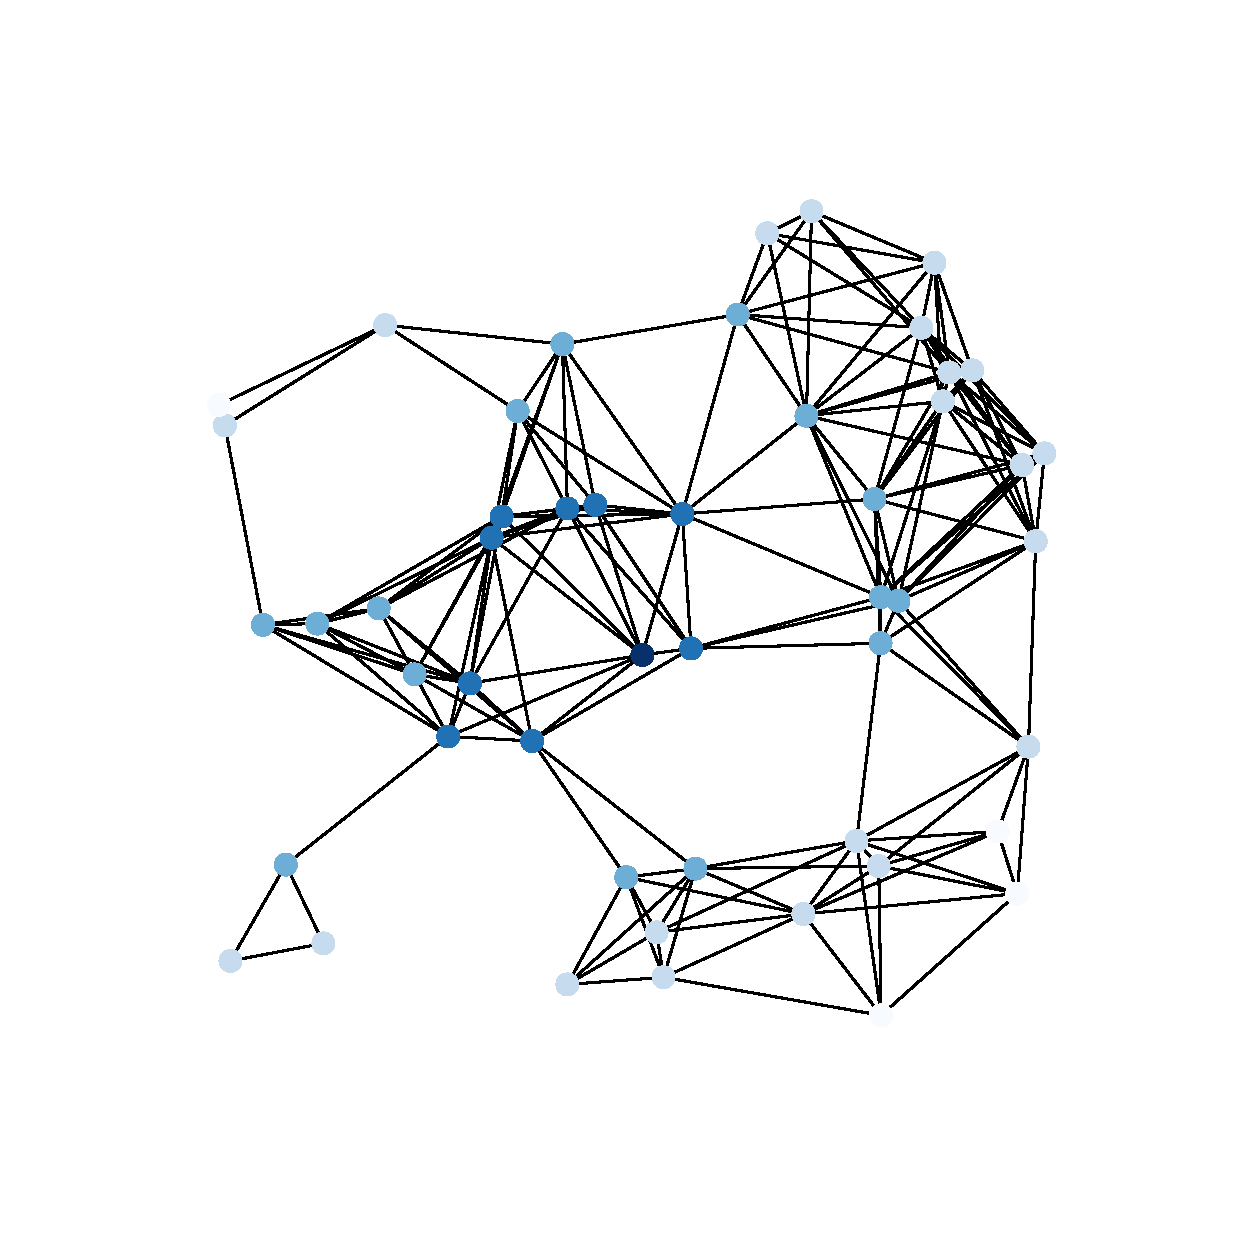
\includegraphics[width=60mm]{./a3g2}}
\subfigure[Grafo 3]{\includegraphics[width=60mm]{./a3g3}}
\subfigure[Grafo 4]{\includegraphics[width=60mm]{./a3g4}}
\subfigure[Grafo 5]{\includegraphics[width=60mm]{./a3g5}}
\caption{Centralidad de cercanía}
\label{figure4}
\end{figure}

\subsection*{Exentricidad}
La figura \ref{figure5} colorea los nodos dependiendo su valor de exentricidad, es decir, entre más obscuro es el nodo, quiere decir que tiene una exentricidad mayor, por lo que por ese nodo, pasan las distancias máximas mas grandes.

\begin{figure}[H]
\centering
\subfigure[Grafo 1]{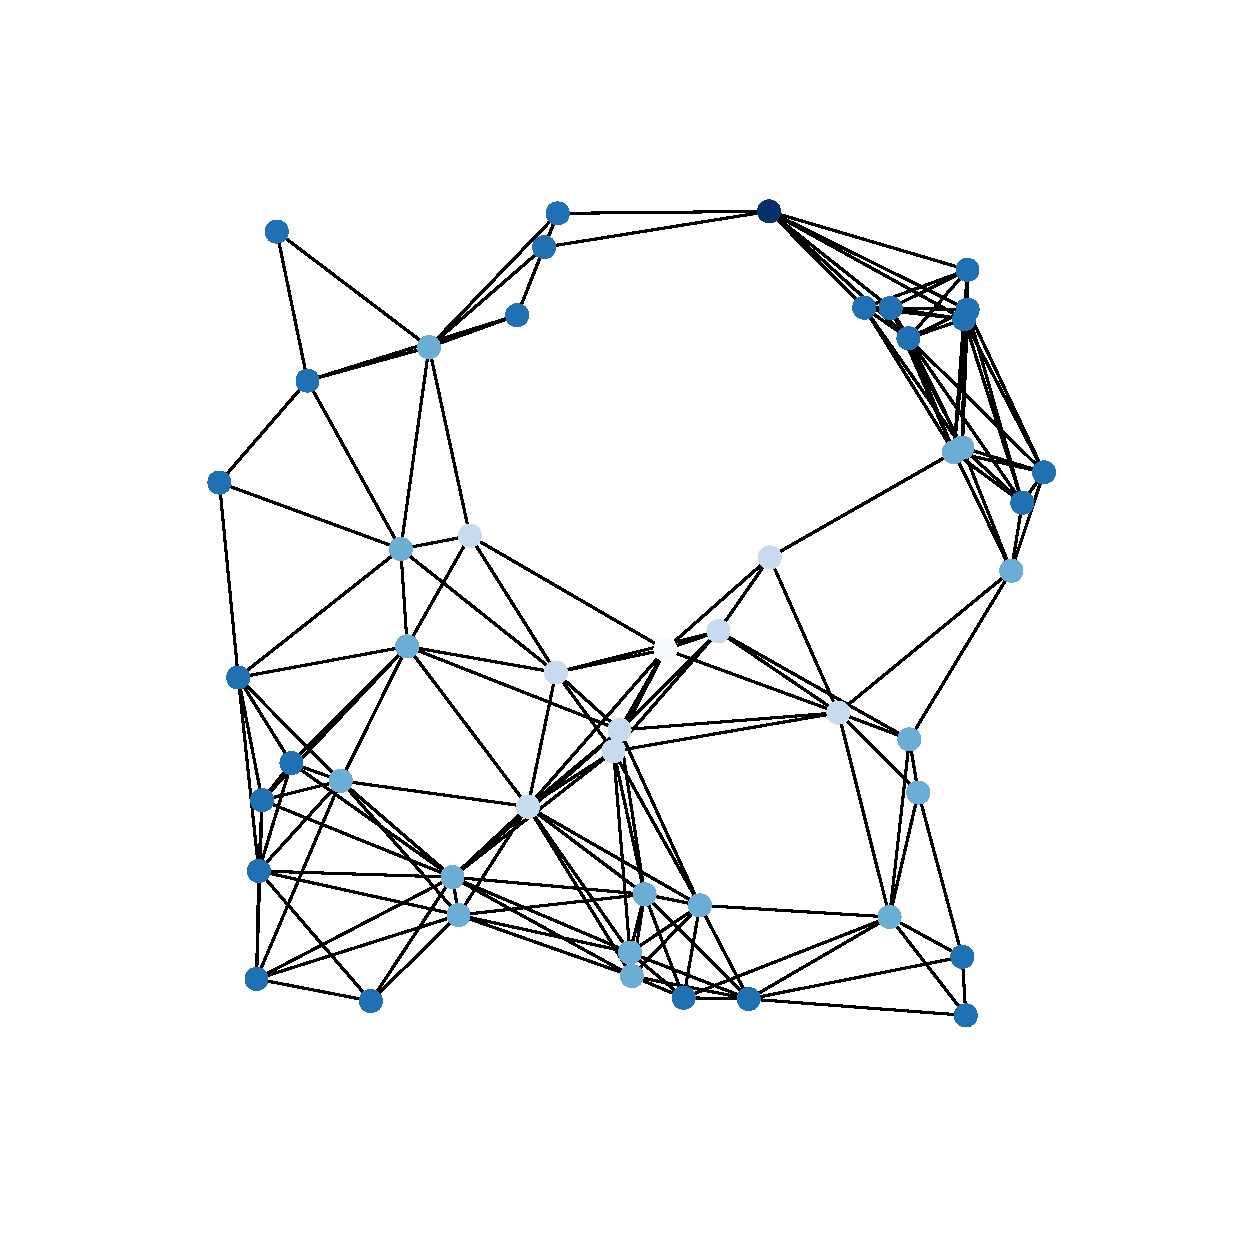
\includegraphics[width=60mm]{./a5g1}}
\subfigure[Grafo 2]{\includegraphics[width=60mm]{./a5g2}}
\subfigure[Grafo 3]{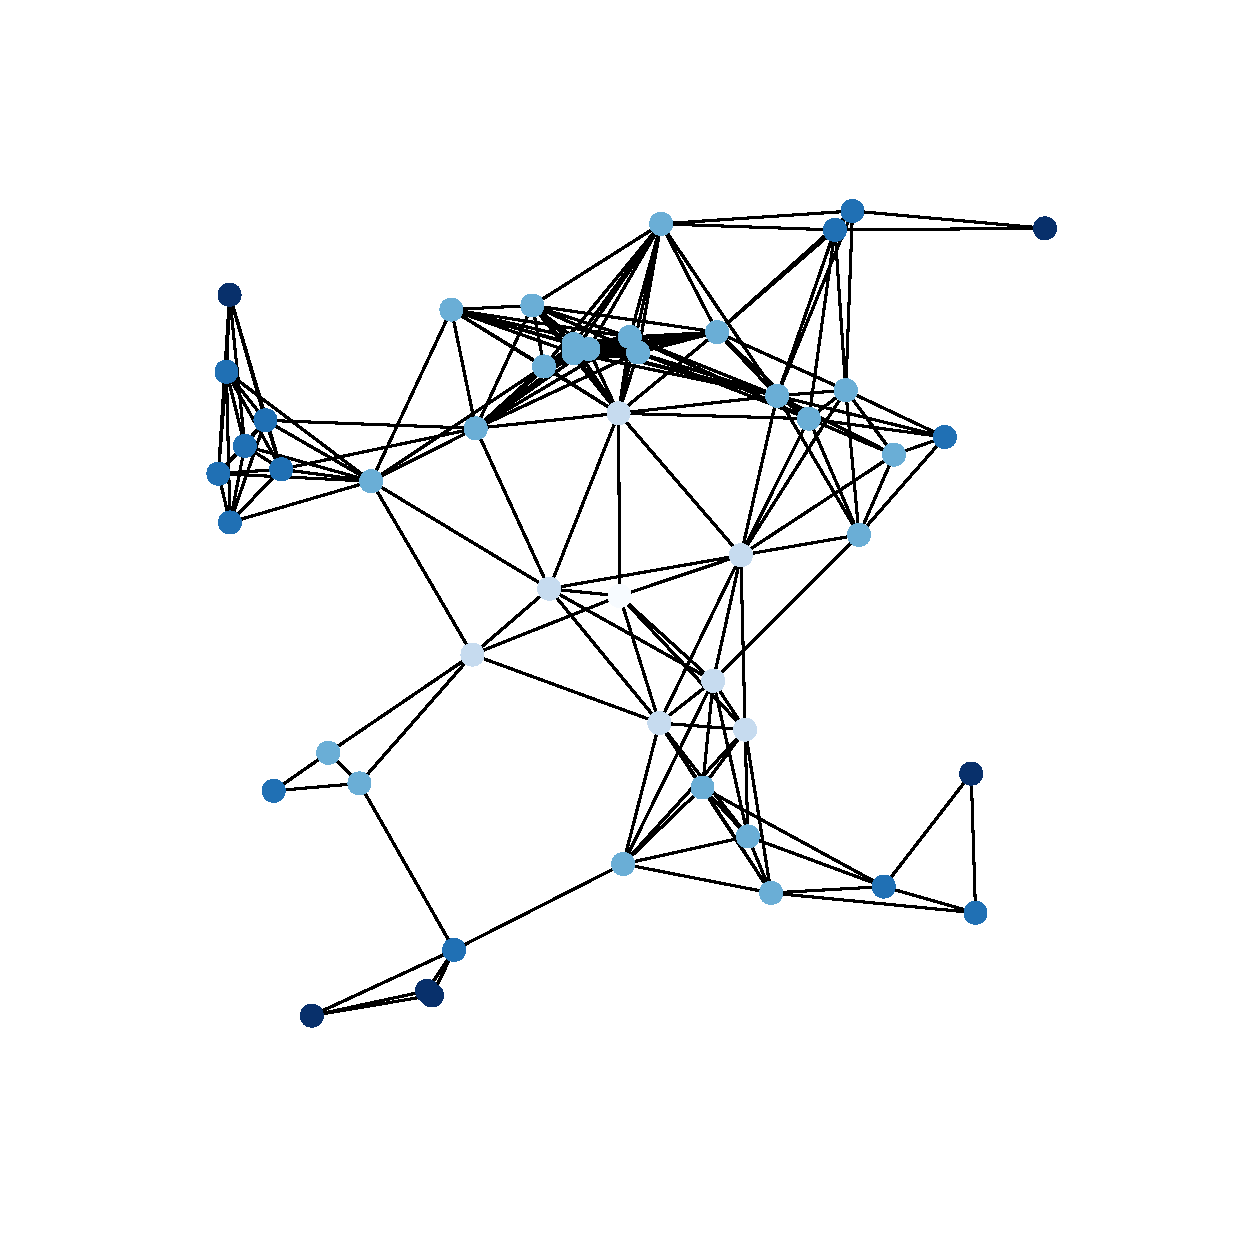
\includegraphics[width=60mm]{./a5g3}}
\subfigure[Grafo 4]{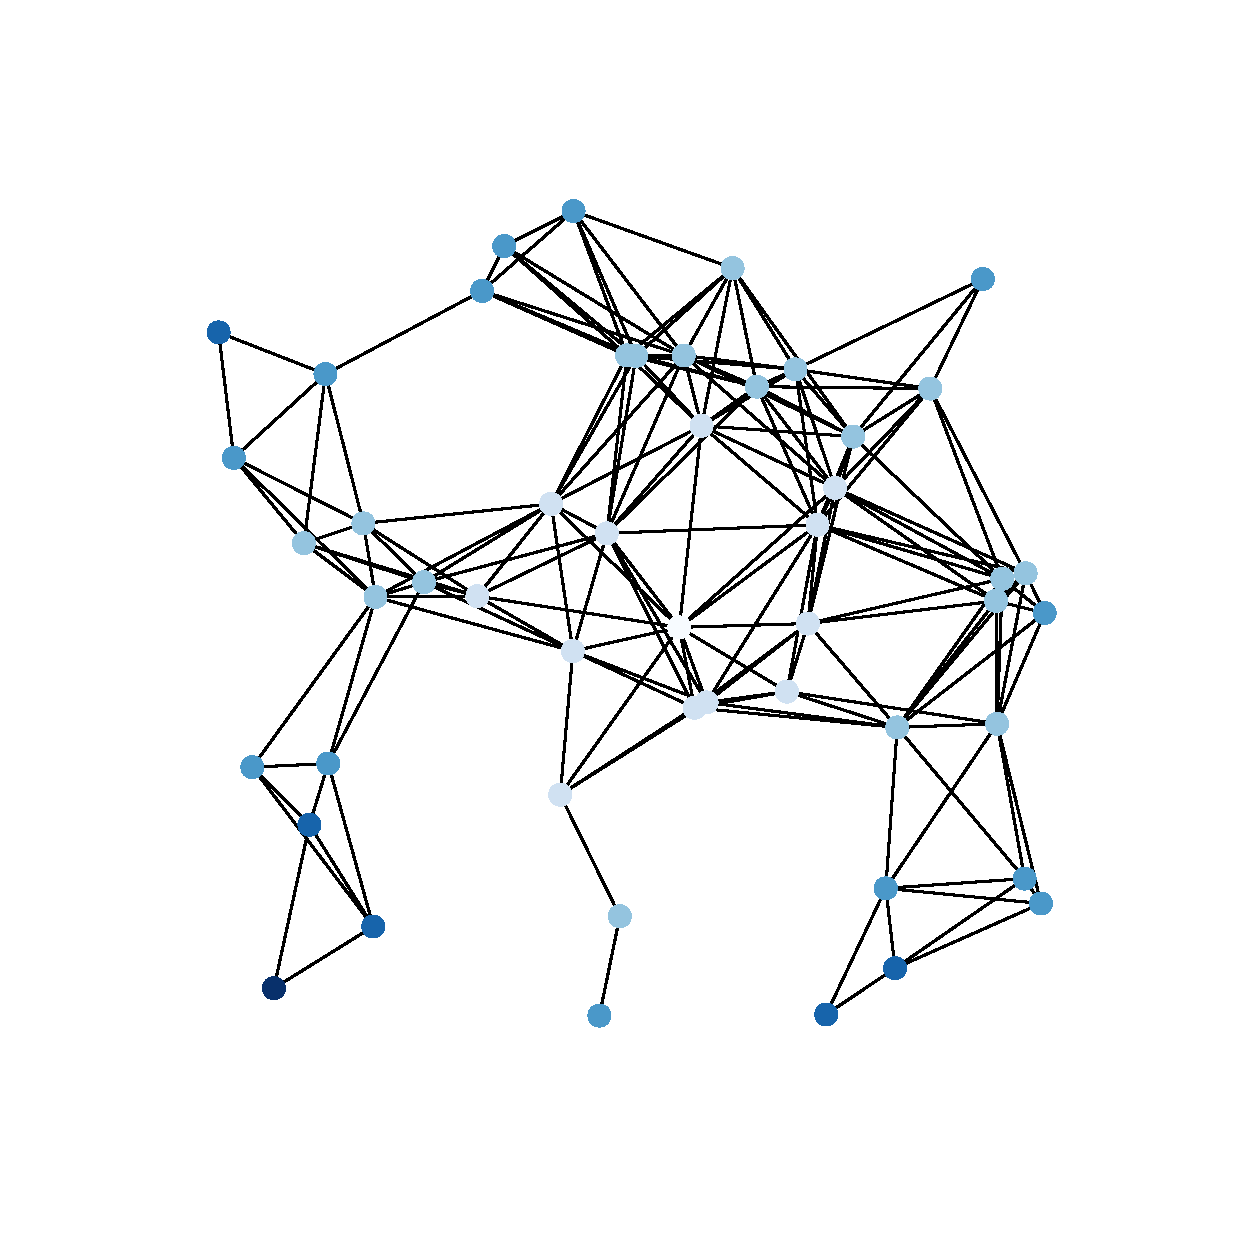
\includegraphics[width=60mm]{./a5g4}}
\subfigure[Grafo 5]{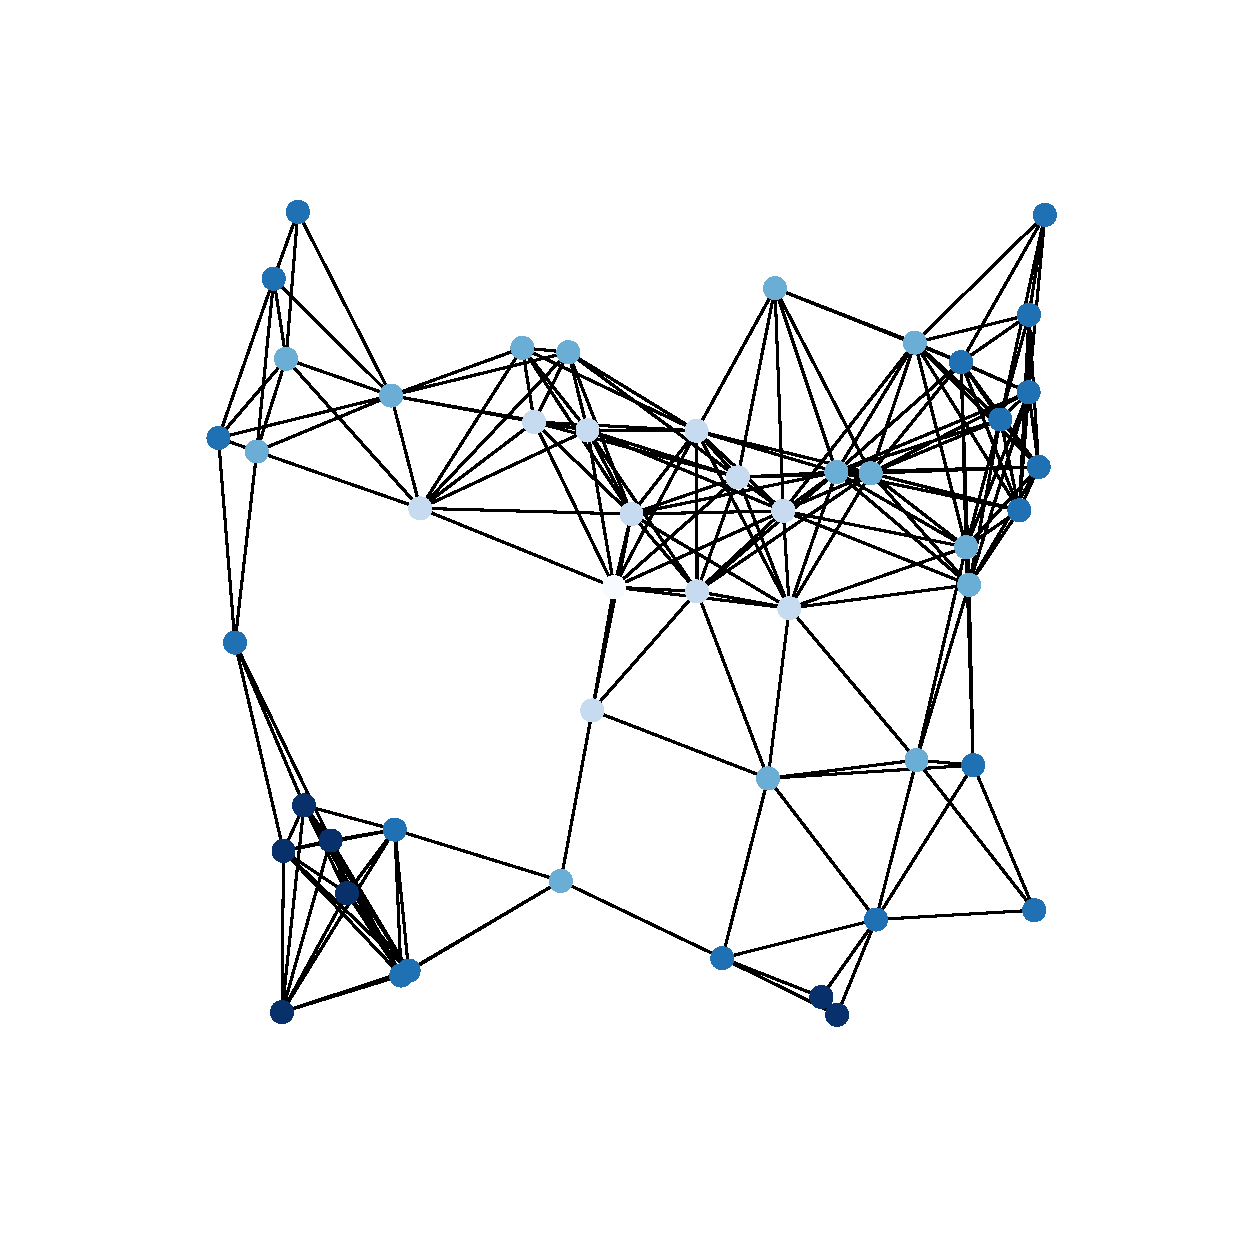
\includegraphics[width=60mm]{./a5g5}}
\caption{Exentricidad}
\label{figure5}
\end{figure}

A continuación se muestran los diagramas de caja y bigotes para los tiempos individuales de los cinco grafos utilizados al ejecutar las seis características estructurales.

\begin{figure}[H]
\centering
\includegraphics[width=120mm]{boxplot1}
\label{figure7}
\end{figure}

\begin{figure}[H]
\centering
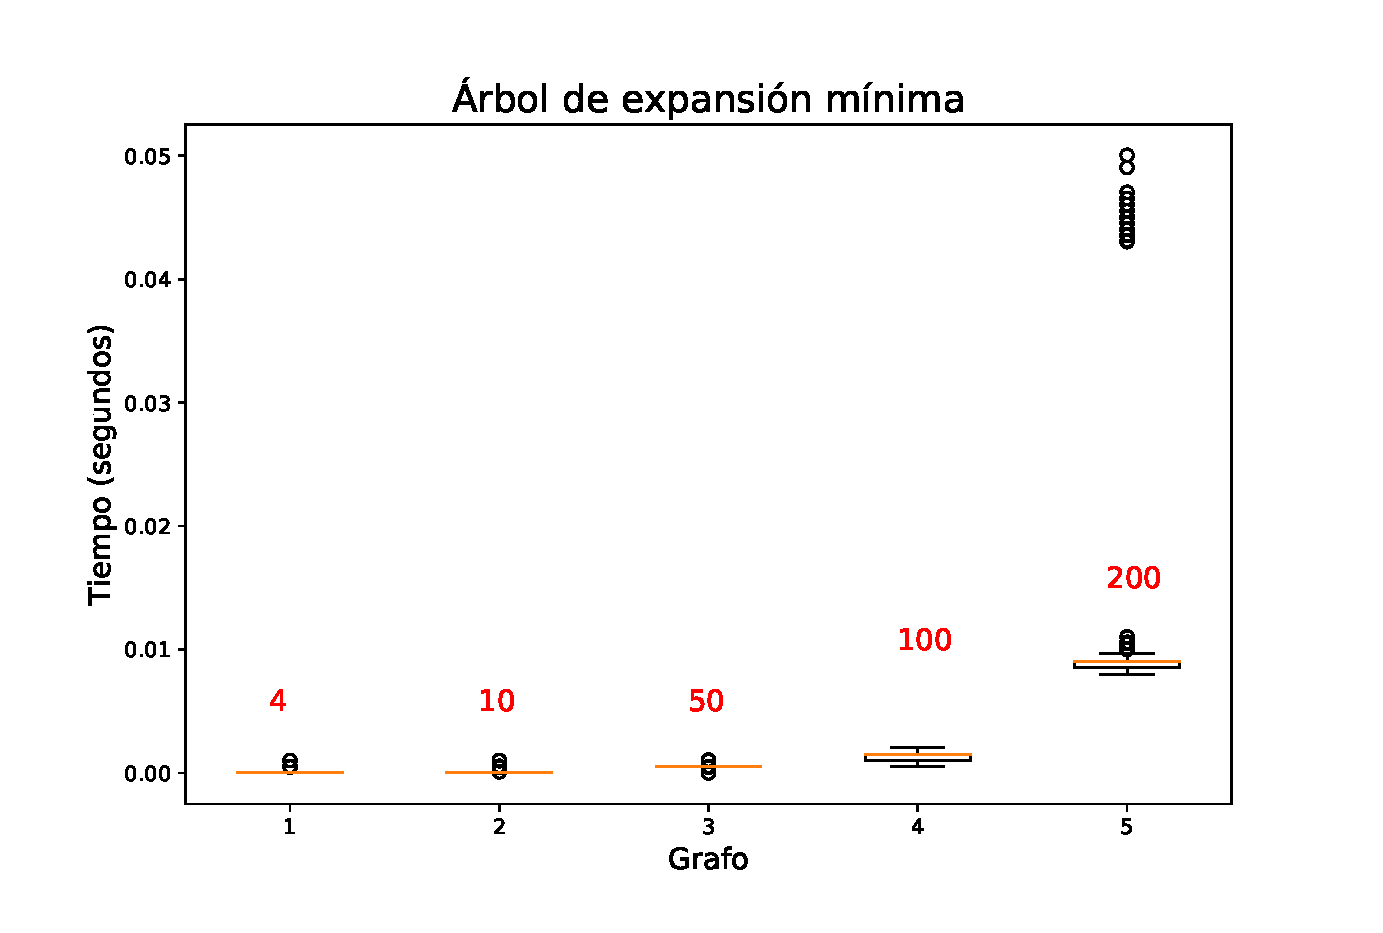
\includegraphics[width=120mm]{boxplot2}
\label{figure7}
\end{figure}

\begin{figure}[H]
\centering
\includegraphics[width=120mm]{boxplot3}
\label{figure7}
\end{figure}

\begin{figure}[H]
\centering
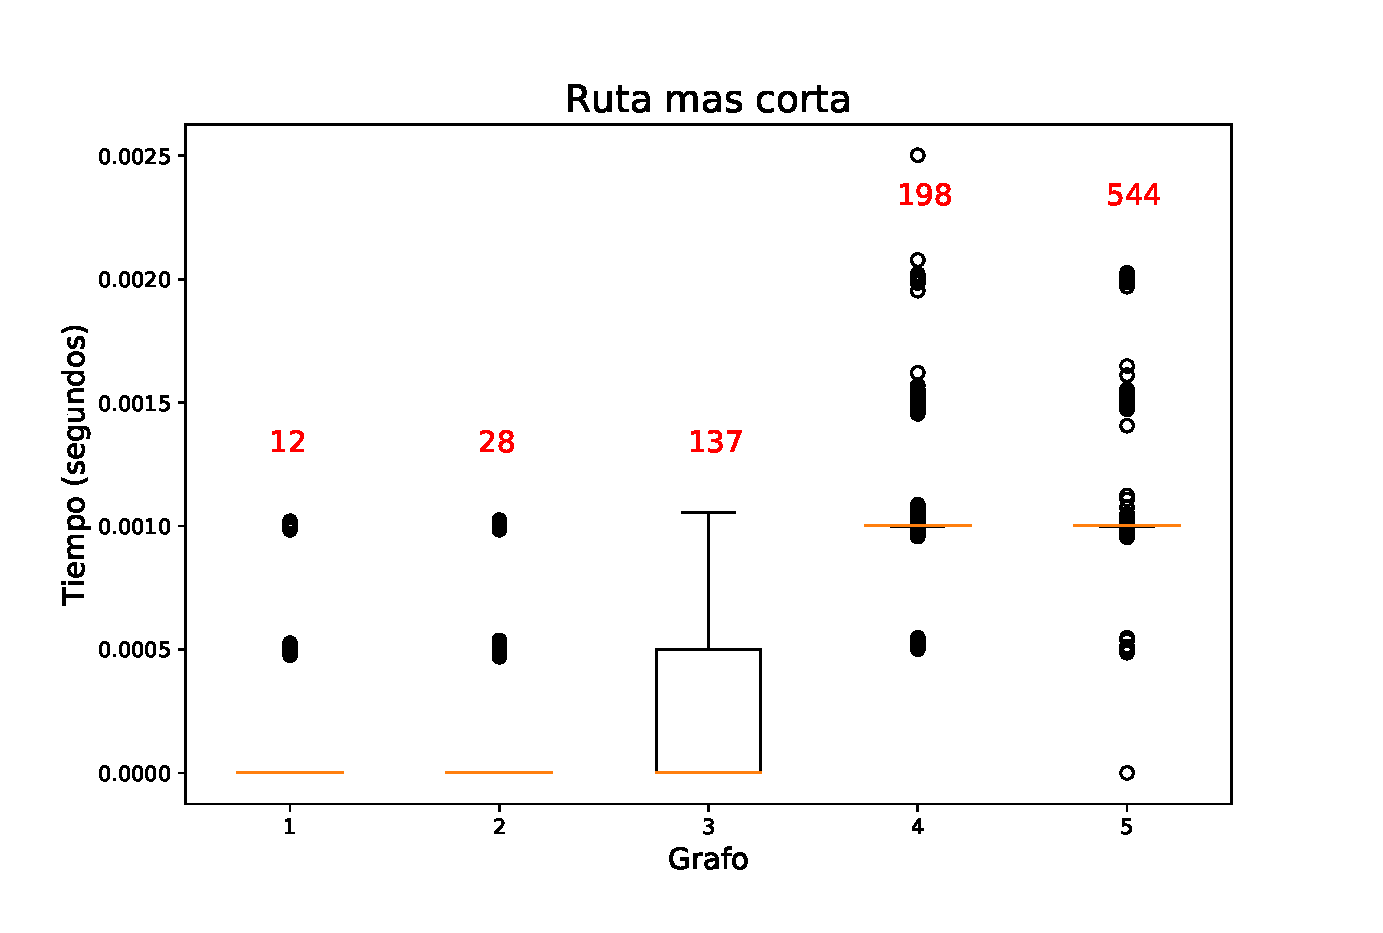
\includegraphics[width=120mm]{boxplot4}
\label{figure7}
\end{figure}

\begin{figure}[H]
\centering
\includegraphics[width=120mm]{boxplot5}
\label{figure7}
\end{figure}

\begin{figure}[H]
\centering
\includegraphics[width=120mm]{boxplot6}
\label{figure7}
\end{figure}


\begin{figure}[H]
\centering
\includegraphics[width=120mm]{mf}
\caption{Grafos contra Valor óptimo} 
\label{figure8}
\end{figure}


\subsection*{Conclusiones}
De los diagramas de caja y bigote se puede apreciar estas características de los nodos no afectan al tiempo de ejecución del algoritmo seleccionado, sin embargo al ver la figura \ref{figure8}, se puede apreciar que al valor del óptimo si.

Si vemos las características en los nodos selecionados como fuente y sumidero podemos ver que los nodos que cumplen las características del nodo fuente y nodo sumidero del grafo 3, resultan ser buenos nodos fuentes y buenos sumideros, ya que el valór del flujo máximo es mayor. Por otro, los nodos que cumplen las características del nodo fuente y nodo sumidero del grafo 1, sería mejor no usar como ninguno si uno busca obtener un alto flujo. Para ambos casos de nodos fuente y sumidero el tiempo de ejecución del algoritmo es rápido. 


\bibliographystyle{unsrt}
\bibliography{biblio}
\nocite{*}


\end{document}